The notion of global semantics\footnote{It defines the full joint distribution as the product of local conditional probability distributions.} describes what a Bayesian network means.
The next step is to explain how to construct a Bayesian network in such a way that the resulting joint distribution is a good representation of a given domain. \vspace{3.5pt}

Another clue about the global semantics is that the Bayesian network is a correct representation of the domain only if each node is conditionally independent
of its predecessors in the node ordering, given its parents. We can satisfy this condition with this methodology:
\begin{enumerate}
    \item First determine the set of variables that are required to model the domain. Order them, ${X_1, \dots, X_n}$. Any order will work, but the resulting network will be more compact if the variables are ordered such that causes precede effects.
    \item For each random variable defined do these actions:
    \begin{itemize}
        \renewcommand{\labelitemi}{-} 
        \item Choose, from $X_1, \dots, X_{i-1}$ a minimal set of parents for $X_i$, such the global semantics equation is satisfied.
        \item For each parent insert a link from it to $X_i$.
        \item Define the conditional probability table.
    \end{itemize}
\end{enumerate}
Intuitively, the parents subset of node $X_i$ should contain all the nodes in the set $X_1, \dots, X_n$ that directly influence $X_i$. This choice of parents guarantees the global
semantics:
\begin{center}
    $\mathbf{P}(X_1, \dots, X_n)$
    
    $ = \prod_{i=1}^{n} \mathbf{P}(X_i|X_1, \dots, X_i-1)$

    $= \prod_{i=1}^{n} \mathbf{P}(X_i|Parents(X_i))$
\end{center}
\begin{example}
    i.e. Let's construct a Bayesian network that help us win a prize. \vspace{3.5pt}

    We're guests on a TV game show. We stand in front of three closed doors. A prize hides behind one of them. We choose the door on the left. At this point, the host,
    who knows where prize is, opens the middle door, to reveal it is empty. We are offered to modify our choice. Should we? \vspace{7pt}

    The necessary nodes to model the domain are: \textit{Guest}, \textit{Host} and \textit{Prize}. \vspace{3.5pt}

    We can say that \textit{Guest} has a direct influence on \textit{Host}, but at the same time it doesn't happens between \textit{$Guest \rightarrow Prize$},
    because he don't know where is located the amount of money. So he has not an influence on \textit{Prize}, cannot be insert a link between them. However, the \textit{Prize}
    has a direct influence on \textit{Host}. The final result it's a \textit{v-structure}, where \textit{Host} is the same child either for \textit{Guest} and \textit{Prize}. \vspace{3.5pt}
    
    In probabilistic terms, it could be described as: \vspace{3.5pt}
    
    $P(P) = P(P|G) \implies P \perp G$

    $P(H) \neq P(H|G)$

    $P(H|G) \neq P(H|G, P)$
\end{example}
We can get a quite compact network only if we choose the node ordering well. What happens if we choose a strange order? Consider the Burglary example again.
\begin{example}
    Suppose we decide to
    order the nodes as follows:
    \begin{center}
        $MaryCalls, JohnCalls, Alarm, Burglary, Earthquake$
    \end{center}
    We then get a more complicated network shown as below. \vspace{3.5pt}
    \begin{center}
        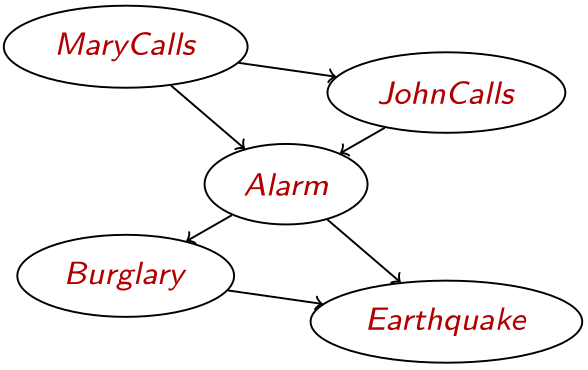
\includegraphics[width=0.5\textwidth]{img/img6.png}
    \end{center} \vspace{3.5pt}
    The process goes as follows:
    \begin{enumerate}
        \item \textit{MaryCalls}: first node, no parents, it is like a \textit{prior probability}.
        \item \textit{JohnCalls}: if Mary calls, probably the alarm has gone off, which would make it more likely John calls. \textit{JohnCalls} needs \textit{MaryCalls} as parent.
        \item \textit{Alarm}: clearly, if both call, it is more likely that the alarm has gone off. \textit{Alarm} needs \textit{MaryCalls} and \textit{JohnCalls} as parents nodes.
        \item \textit{Burglary}: if we know the alarm state, then the call from Mary or John doesn't tell us anything about the Burglary: 
        \begin{center}
            $\mathbf{P}(Burglary|Alarm, JohnCalls, MaryCalls) = \mathbf{P}(Burglary|Alarm)$    
        \end{center}
        Hence we need just \textit{Alarm} as parent.
        \item \textit{Earthquake}: if the alarm is on, it is more likely that there has been an earthquake. But if we know that there has been a Burglary, then that explain the alarm, so the probability of an earthquake would decrease. Hence, we need both \textit{Alarm} and \textit{Burglary} as parent.
    \end{enumerate} \vspace{3.5pt}

    The resulting network has two more links than the original one and requires three more probabilities to be specified. What's worse, some of the links represent strange relationships
    that require difficult probability judgments. 
\end{example}
If we try to build a Bayesian network by the \textbf{diagnostic direction}, from effects to causes, we end up having to specify additional dependencies between independent causes. If we use the \textbf{causal direction}, we end up having to 
specify fewer numbers, and the network seems to be more easier to handle.